\documentclass{article}

\usepackage{amsmath}
\usepackage{amsthm}
\usepackage{amssymb}
\usepackage{bbm}
\usepackage{fancyhdr}
\usepackage{listings}
\usepackage{cite}
\usepackage{graphicx}
\usepackage[margin=1cm]{caption}
\usepackage{subcaption}
\usepackage{tcolorbox}
\usepackage{color, wrapfig, float, tcolorbox}
\usepackage[shortlabels]{enumitem}
\definecolor{editorGray}{rgb}{0.95, 0.95, 0.95}
\usepackage{hyperref}

\lstset{%
    % Basic design
    backgroundcolor=\color{editorGray},
    basicstyle={\small\ttfamily},   
    frame=l,
    % Line numbers
    xleftmargin={0.75cm},
    numbers=left,
    stepnumber=1,
    firstnumber=1,
    numberfirstline=false,
    }
\lstset{
    literate={~} {$\sim$}{1}
}

\newenvironment{claim}[1]{\par\noindent\underline{Claim:}\space#1}{}
\newenvironment{claimproof}[1]{\par\noindent\underline{Proof:}\space#1}{\hfill $\blacksquare$}

\oddsidemargin 0in \evensidemargin 0in
\topmargin -0.5in \headheight 0.25in \headsep 0.25in
\textwidth 6.5in \textheight 9in
\parskip 6pt \parindent 0in \footskip 20pt

% set the header up
\fancyhead{}
\fancyhead[L]{Stanford Aeronautics \& Astronautics}
\fancyhead[R]{Fall 2021}

%%%%%%%%%%%%%%%%%%%%%%%%%%
\renewcommand\headrulewidth{0.4pt}
\setlength\headheight{15pt}

\usepackage{outlines}

\usepackage{xparse}
\NewDocumentCommand{\codeword}{v}{%
\texttt{\textcolor{blue}{#1}}%
}
\usepackage{gensymb}

\newcommand{\ssmargin}[2]{{\color{blue}#1}{\marginpar{\color{blue}\raggedright\scriptsize [SS] #2 \par}}}


\setlength{\parindent}{0in}

\title{AA 274A: Principles of Robot Autonomy I \\ (in-person) Section 9: Coordinate Frame \& Transforms}
\date{}

\begin{document}

\maketitle
\pagestyle{fancy}

\begin{wrapfigure}{r}{0.25\textwidth}
\centering
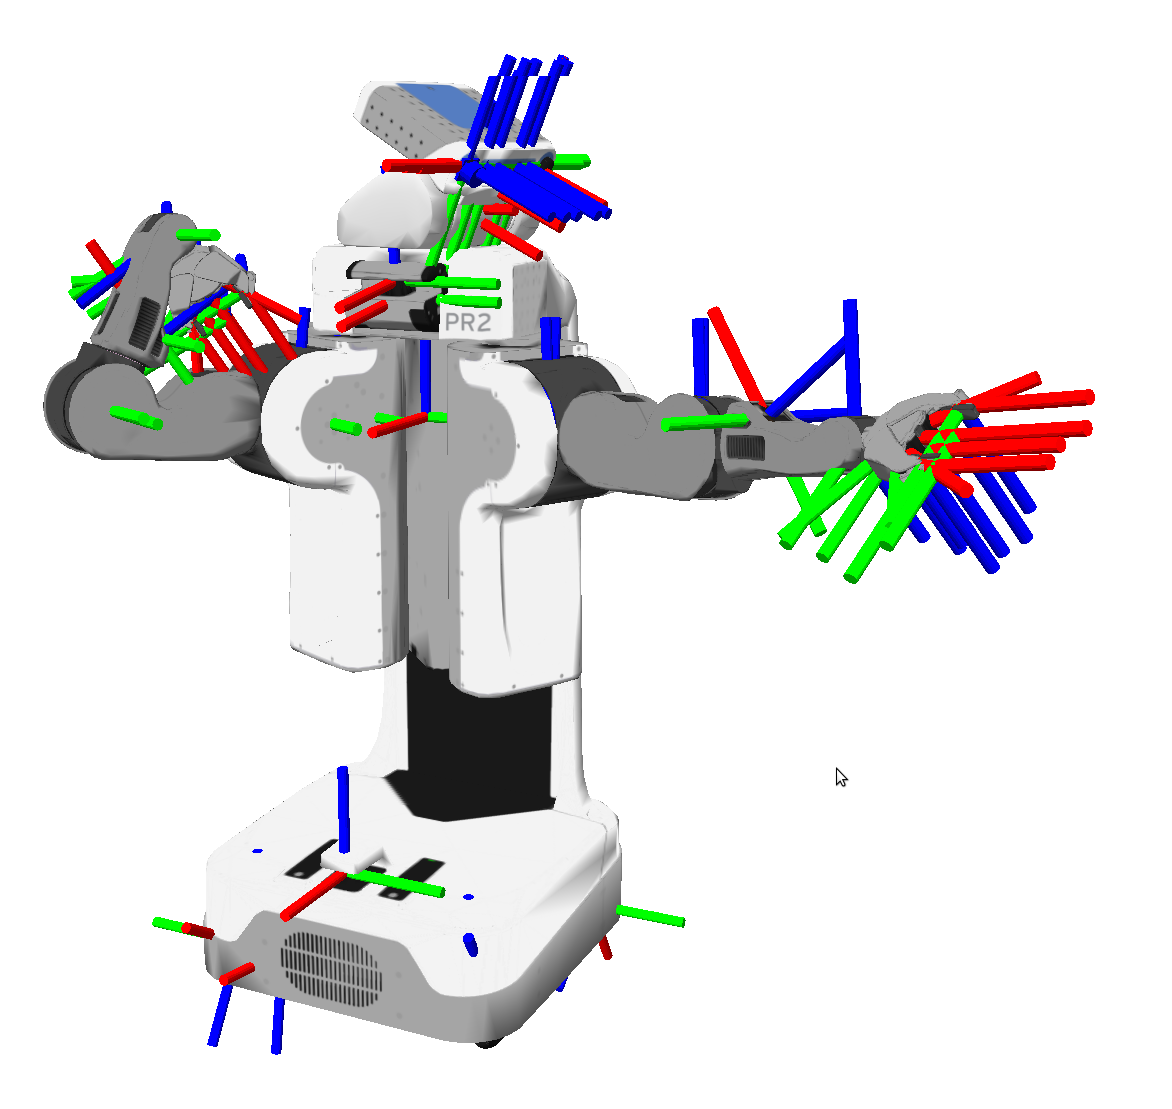
\includegraphics[width=0.25\textwidth]{s9/figs/ros_tf_image.png}
\caption{Robots can have very many coordinate frames and transforming between them should be painless. \href{http://wiki.ros.org/tf2}{wiki.ros.org/tf2}}
\end{wrapfigure}

\section{Coordinate Frames}

Using many coordinate frames on a robot makes specifying positions and orientations of various objects much more natural. Some examples include: (i) the robot drives around and rotates relative to its initial position, (ii) the map stays fixed and maps the initial robot position onto it, (iii) the LIDAR and the camera observe points relative to their own position, (iv) the wheels of the robot rotate around their attachment point on the robot and (v) a robotic arm mounted on top a robot has its based located relative to the robot and its tip located relative to the its base.

Going through these examples: (i) the translation and rotation from the initial robot pose to the current pose is natural, (ii) the initial robot position is naturally expressed relative to the map's origin, (iii) the LIDAR and camera might be aligned with the robot's pose, but they are most likely translated, a little away from the definitional center of the robot, (iv) the wheels of the robot continuously rotate, but around a fixed point on the robot, (v) robotic arm moves and contains at least two frames.

In principle, if we know any transform we know (a) the inverse transform and (b) we know any transform between any two frames if all intermediate frames have their a one-directional transform defined between them.

ROS defines only two types of pairwise coordinate frame transforms: normal and static. Normal transforms assume that the transform between the two frames varies in time and so needs to be constantly updated and the static transform assumes that the transform does not change with time. 

\begin{tcolorbox}[title=ROS Transforms Takeaways]
The static transform can be defined once and can be looked up for any time. The normal transform must be constantly published via the transform publisher and can be looked up for the time range when it was published.

ROS uses the \texttt{tf2\_ros} package to look up transforms. \texttt{tf2\_ros} requires creating a buffer that listens to all transforms since it was created, but performs transform math, for the lookup, based on the transform history recorded in the lookup. Most often, only the latest transform is taken---when looking up a transform for ``now" (a current transform).
\end{tcolorbox}

Figure \ref{fig:convention} contains the common conventions for coordinate frame names. Figure \ref{fig:frames} contains all coordinate frames for the virtual ASL turtlebot visualized as a graph. The arrows show the direction of the defined transform, but the transform can be obtained in either direction. Because all coordinate frames should be connected via a known transform to one other frame, a transformation between any two coordinate frames can be computed easily.

\newpage

Before beginning launch the the project launch file (with a Gazebo simulation).

\texttt{roslaunch asl\_turtlebot project.launch}

\textbf{Problem 1:} Create a function which build a TransformStamped message from a given translation and a yaw.

Hint: Look up the definition of the TransformStamped message.

Hint: Yaw is the third Euler angle in the roll-pitch-yaw convention most commonly used in ROS.

Hint: take a look at \texttt{tf\_conversions.transformations.quaternion\_from\_euler}.

\textbf{Problem 2:} Create a publisher that publishes a static transform between the map origin and the location of a static ``object", 3 meters in $x$ and $0.1$ m in $z$ directions.

Hint: take a look at \texttt{tf2\_ros.StaticTransformBroadcaster} and \texttt{sendTransform} method of that class.

\textbf{Problem 3:} Create a publisher that publishes a normal transform between the map origin and the location of a moving ``object" that rotates around the map origin at 1 rad/s at a radius of $5$ m.

Hint: take a look at \texttt{tf2\_ros.TransformBroadcaster} and \texttt{sendTransform} method of that class.

\textbf{Problem 4:} Look up the transform between the robot and the static object from Problem 2.

Hint: take a look at creating a \texttt{tf2\_ros.Buffer}.

Hint: take a look at creating a \texttt{tf2\_ros.TransformListener}.

Hint: take a look at looking up a transform with the \texttt{lookup\_transform} method of the \texttt{tf2\_ros.Buffer} class.

\textbf{Problem 5:} Look up the transform between the robot and the moving object from Problem 3.

\newpage
\begin{figure}[H]
\centering
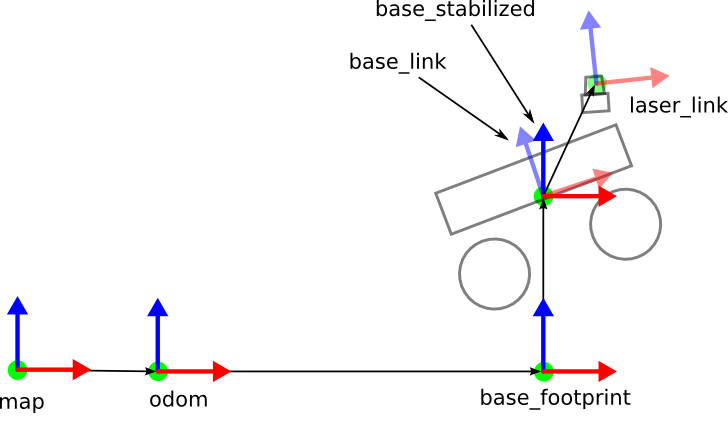
\includegraphics[width=0.5\linewidth]{s9/figs/coordsystems_img.png}
\caption{\texttt{map} - origin of the map coordinate frame. \texttt{odom} - robot pose on initialization. \texttt{base\_footprint} - current robot pose mapped on the ground plane. \texttt{base\_link} - full robot pose. 
\href{http://wiki.ros.org/hector\_slam/Tutorials/SettingUpForYourRobot}{wiki.ros.org/hector\_slam/Tutorials/SettingUpForYourRobot}
\label{fig:convention}
}

\end{figure}
\begin{figure}[H]
\centering
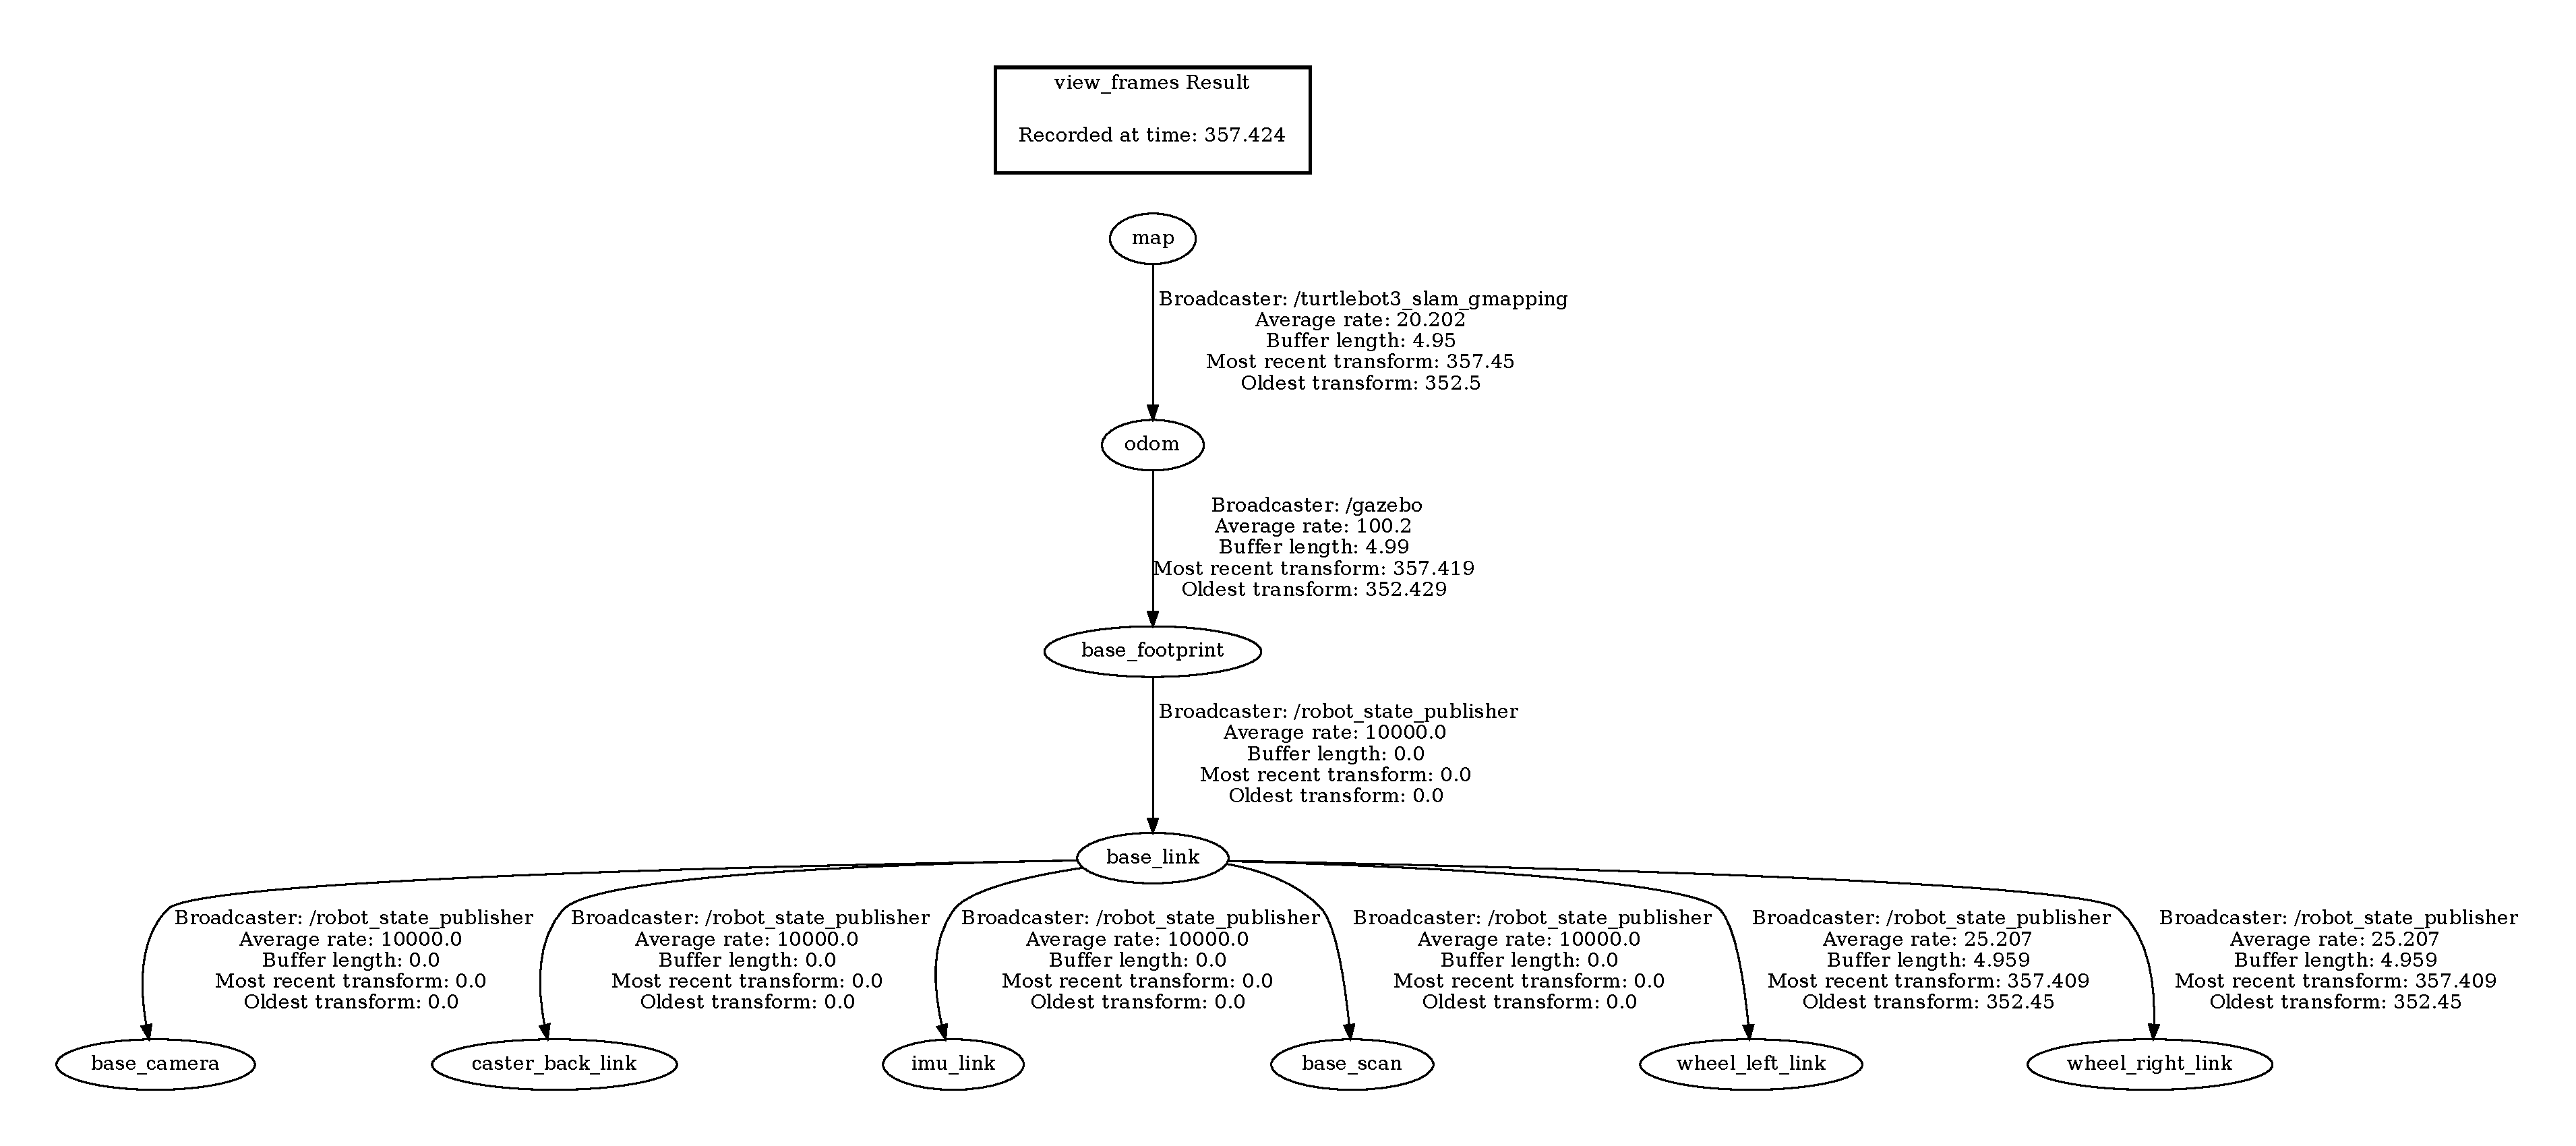
\includegraphics[width=\linewidth]{s9/figs/frames.pdf}
\caption{An example of the coordinate frame graph for the virtual ASL turtlebot launched from the \texttt{project.launch} file.}\label{fig:frames}
\end{figure}


\end{document}